\section{¿Aumenta el acceso a internet la variabilidad de la nota?}

Internet puede ser una poderosa herramienta para el aprendizaje de los alumnos, aportando una cantidad inmensurable de materiales didácticos de forma gratuita. Sin embargo, también trae consigo las redes sociales, a las cuales se les atribuye varios efectos adversos como la perdida la de atención.
\begin{equation*}
    \begin{split}
        & X \equiv \text{Nota final de los alumnos con acceso a internet}\\
        & Y \equiv \text{Nota final de los alumnos sin acceso a internet}
    \end{split}
\end{equation*}
    
En nuestros datos vemos que las varianzas muestrales varían en una unidad. Veremos si estas observaciones son atribuibles al azar.
\begin{equation*}
    \begin{split}
        & S_x^2 = 20.92\\
        & S_{y}^2 = 19.82
    \end{split}
\end{equation*}

Antes de elegir el test, debemos comprobar la normalidad de los datos para ver si elegimos un contraste paramétrico o no paramétrico.

\begin{figure}[H]
    \begin{center}
        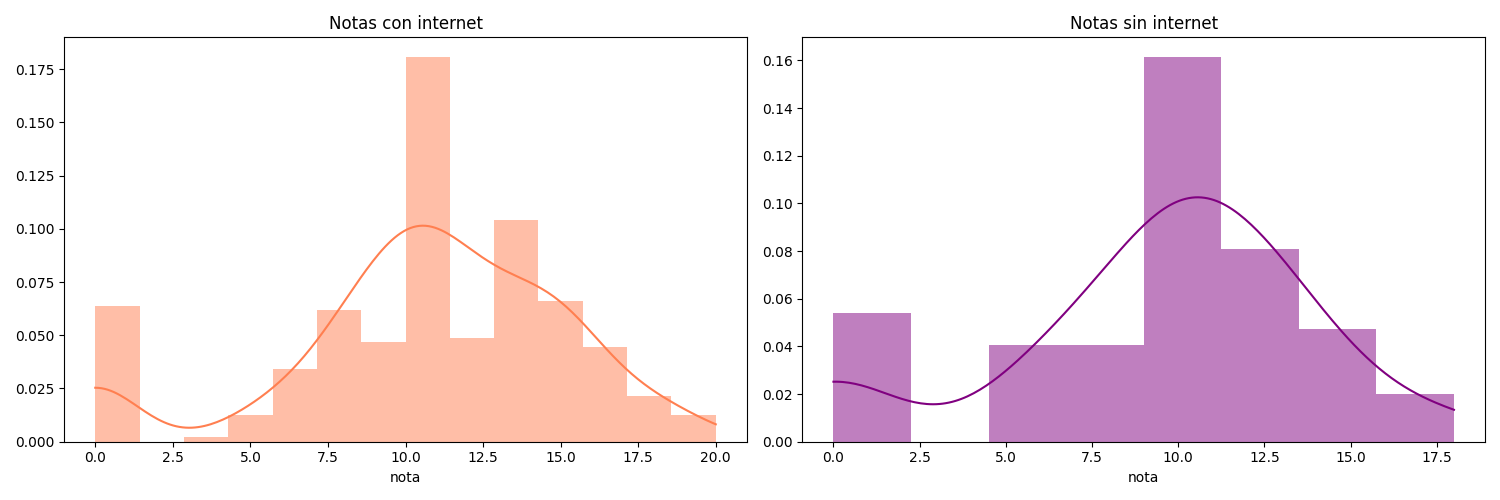
\includegraphics[width=1\textwidth]{figures/dist-notas-internet.png}
    \end{center}
    \caption{Gráficos de distribución de las notas finales con y sin internet}\label{fig:dist-notas-internet}
\end{figure}

Como en casos anteriores, utilizaremos el test de Ómnibus d´Agostino.
\begin{equation*}
    \begin{split}
        & K_{x}^2 = 28.77 \Rightarrow \text{p-valor} = P(K^2 > 28.77) \approx 0\\
        & K_{y}^2 = 6.15 \Rightarrow \text{p-valor} = P(K^2 > 6.15) = 0.046
    \end{split}
\end{equation*}

En ambos casos, al $5 \%$, rechazaríamos la hipótesis nula de normalidad.

Aunque nuestros datos tienen asimetría negativa moderada y son muestras grandes, el contraste $F$ de diferencia de varianzas es especialmente sensible a la no-normalidad de los datos. Por lo tanto, viendo que los datos muestran evidencias suficientes como para rechazar la normalidad, nos decantaremos por un test no-paramétrico.
\begin{equation*}
    \begin{split}
        & \gamma_{1}(x) = \frac{\sum_{i=1}^{n}(x_i - \bar{x})^3}{n \cdot s^3} = -0.75\\
        & \gamma_{1}(y) = \frac{\sum_{i=1}^{n}(y_i - \bar{y})^3}{n \cdot s^3} = -0.71
    \end{split} 
\end{equation*}

Aplicaremos un contraste de Levene de igualdad de varianzas.

\begin{itemize}
    \item \textbf{Hipótesis nula ($H_0$)}: $\sigma_{x}^2 = \sigma_{y}^2$ (no existen diferencias significativas entre la varianza de las notas de los alumnos con internet y los alumnos sin internet)
    \item \textbf{Hipótesis alternativa ($H_a$)}: $\sigma_{x}^2 \neq \sigma_{y}^2$ (existen diferencias significativas entre la varianza de las notas de los alumnos con internet y los alumnos sin internet)
\end{itemize}

Al calcular el estadístico de contraste $W$ obtenemos los siguientes resultados:
\begin{equation*}
    W = 0.17 \Rightarrow \text{p-valor} = P(F_{k-1,N-k} > W) = P(F_{1, 393} > 0.17) = 0.68
\end{equation*}

Entonces, como hemos obtenido un p-valor alto, los datos son compatibles con la hipótesis nula de igualdad de varianzas. Los datos no muestran evidencias suficientes como para rechazar que las varianzas en las notas de los alumnos con y sin internet sean iguales. Por lo tanto, aceptaremos que el hecho de tener internet no influye en la variabilidad de la nota.
